\documentclass[a4paper]{article}

\usepackage[utf8]{inputenc}
\usepackage[L7x]{fontenc}
\usepackage[lithuanian]{babel}
\usepackage{lmodern}
\usepackage{graphicx}
\usepackage{amsmath}
\usepackage{animate}
\usepackage{verbatim}
\usepackage{pgfplots}
\usepackage{hyperref}
\usepackage{empheq}
\usepackage[many]{tcolorbox}
\usepackage{mdframed}
\usepackage{framed}
\usepackage{mdframed}
\usepackage{indentfirst}
\usepackage{tasks}
\usepackage{cancel}
\usepackage{enumitem}
\usetikzlibrary{arrows} %geogebra
\usepackage[top=2cm, bottom=2cm, left=2cm, right=2cm, footskip=1cm, a4paper]{geometry}
\newcommand{\tbf}[1]{\textbf{#1}}
\newcommand{\tit}[1]{\textit{#1}}
\newcommand{\hitem}[1]{\item[\stepcounter{enumi}\href{#1}{\theenumi.}]} %Linked item 

\newcounter{nameOfYourChoice}
\newcommand{\save}{\setcounter{nameOfYourChoice}{\value{enumi}}} %saves number of item
\newcommand{\resume}{\setcounter{enumi}{\value{nameOfYourChoice}}} %resumes the last saved item

\begin{document}
\section*{Kaip mokytis trigonometriją}
Vadovėlis pilną funkcionalumą išlaiko tik atidarant jį su Adobe Acrobat. Tai reiškia, failą naršyklėje neveiks animacijos ir galbūt nuorodos. Norėdami išbandyti pirmo brėžinio funkcijas, turite būti suinstaliavę Geogebra. Norėdami pasitikrinti uždavinių atsakymus, į \href{http://wolframalpha.com}{WolframAlpha} laukelį įveskite komandas 180 degrees, sin(180), sin(pi/4), 4sin(x)*cos(x) ir pan. Hint: paspaudus ant uždavinių pakliūsite į vertingas nuorodas.
\newline
\newline
Kuo šis vadovėlis skiriasi nuo nuobodžių mokyklinių vadovėlių? 
\begin{itemize}
\item Jame yra atsižvelgiama, kad matematinės žinios yra įgyjamos keliais vienas po kito einančiais mokymosi lygmenimis: susipažįstant ir eksperimentuojant su nagrinėjamos sąvokos vaizdiniu, praktikuojantis su aritmetinėmis operacijomis ir galiausiai apibendrinant tą, ką būtina įsiminti, kuo paprastesniu būdu. Todėl temos pristatomos parodant kuriuos keliu visuose lygmenyse reikėtų judėti.
\item Apibendrinimas neįsisavinamas tol, kol nagrinėjami dalykai nepačiupinėjami jūsų pačių. Pratimai čia skirti ne tam, kad išmoktumėte atkartoti į kontrolinius ir egzaminus įeinančias procedūras, o tam, kad įgytumėte patirties, leidžiančios patiems pastebėti kelią, kuriuo reikia eiti atakuojant kontrolinių bei egzaminų uždavinius. Taip didinamas pasitikėjimas savo žiniomis matematikoje ir sumažinamas nuolatinis įgytų žinių užmiršimas.
\item Siūlomi nestandartiniai, efektyvesni metodai spręsti uždaviniams ir įsiminti informacijai.
\end{itemize}
\newpage 
\section{Kampai ir jų trigonometrinės funkcijos}

\subsection{BRĖŽINYS, kuris padeda lengvai įsivaizduoti $\sin x$ ir $\cos x$ funkcijas}

Ant koordinačių plokštumos taško $(0, 0)$ BRĖŽINYJE pavaizduojame vienetinį apskritimą:

\href{run: circlegame.ggb}{\includegraphics[width=0.5\textwidth]{"circlegame".png}}

Šią konstrukciją, paaiškinančią $\sin$ ir $\cos$ prasmę, vadiname trigonometriniu skrituliu.

\begin{mdframed}[backgroundcolor=yellow!50!white]
\begin{itemize}
\item Kampo $A$ sinusą \fbox{$\sin{A}$} nurodo pavaizduoto spindulio šešėlinė dalis Oy ašyje. Konkrečiau: statmens į $y$ pagrindo padėtis $y$ ašyje.
\item Kampo $A$ kosinusą \fbox{$\cos{A}$} nurodo pavaizduoto spindulio šešėlinė dalis Ox ašyje. Konkrečiau: statmens į $x$ pagrindo padėtis $x$ ašyje.
\item Kampo $A$ tangentu \fbox{$\text{tg}{A}$} vadiname santykį $\frac{\sin{A}}{\cos{A}}$. Šis santykis yra būdas apibrėžti, kas yra tangentas.
\item Kampo $A$ kotangentu \fbox{$\text{ctg}{A}$} vadiname santykį $\frac{\cos{A}}{\sin{A}}$. Šis santykis yra būdas apibrėžti, kas yra kotangentas.
\item Sinusas ir kosinusas bet kuriam kampui $A$ yra susieti sąryšiu $$\sin^2{A}+\cos^2{A}=1$$ Tai galioja pagal Pitagoro teoremą.
\end{itemize}
\end{mdframed}

\begin{mdframed}[backgroundcolor=blue!10!white, linewidth=3pt]
\begin{enumerate}
\item Naudodamiesi BRĖŽINIU nustatykite, kokius ženklus įgyja $\sin(\alpha)$ ir $\cos(\alpha)$, kai:
\begin{tasks}(4)
\task $\alpha \in \text{(0°;90°)}$
\task $\alpha \in \text{(90°; 180°)}$
\task $\alpha \in \text{(180°; 270°)}$
\task $\alpha \in \text{(270°; 360°)}$
\end{tasks}
\item Naudodamiesi BRĖŽINIU nustatykite, kaip kinta (auga ar mažėja) $\sin(\alpha)$ ir $\cos(\alpha)$ reikšmės, kai:
\begin{tasks}(2)
\task $\alpha$ auga nuo 0° ligi 90°.
\task $\alpha$ auga nuo 90° ligi 180°.
\task $\alpha$ auga nuo 180° ligi 270°.
\task $\alpha$ auga nuo 270° ligi 360°.
\end{tasks}
\hitem{https://www.wolframalpha.com/input/?i=cos+90} Naudodamiesi BRĖŽINIU nustatykite trigonometrinių funkcijų reikšmes 
\begin{tasks}(3)
\task $\sin{0^o}$ ir $\cos{0^o}$
\task $\sin{90^o}$ ir $\cos{90^o}$
\task $\sin{180^o}$ ir $\cos{180^o}$
\task $\sin{270^o}$ ir $\cos{270^o}$
\task $\sin{360^o}$ ir $\cos{360^o}$
\task $\sin{450^o}$ ir $\cos{450^o}$
\task $\sin{(-90^o)}$ ir $\cos{(-90^o)}$
\task $\sin{(-270^o)}$ ir $\cos{(-270^o)}$
\task $\sin{900^o}$ ir $\cos{900^o}$
\end{tasks}
\save \end{enumerate}
\end{mdframed}
\begin{mdframed}[backgroundcolor=blue!10!white, linewidth=3pt]
\begin{enumerate} \resume
\hitem{https://en.wikipedia.org/wiki/Special\_right\_triangle} Duota, jog stačiojo trikampio įžambinė lygi 1. Abiem iš pavaizduotų atvejų naudodamiesi geometrinėms žiniomis raskite jo likusių kraštinių ilgius:
\begin{tasks}(2)
\task \includegraphics[width=0.2\textwidth]{"454590triangle".png}
\task \includegraphics[width=0.3\textwidth]{"306090triangle".png}
\end{tasks}
\hitem{https://www.wolframalpha.com/input/?i=sin(72)} Patalpinkite šiuos trikampius trigonometriniame skritulyje. Pasinaudodami ankstesnio pratimo rezultatais nustatykite $\cos\text{30°}$, $\cos$ 45°, $\cos$ 60°, $\sin$ 30°, $\sin$ 45°, $\sin$ 60° reikšmes.
\hitem{} Pasinaudodami ankstesnio pratimo išvadomis nustatykite $\text{tg}\text{ 30°}$, $\text{tg}\text{ 45°}$, $\text{tg}\text{ 60°}$, $\text{ctg}\text{ 30°}$, $\text{ctg}\text{ 45°}$, $\text{ctg}\text{ 60°}$ reikšmes.
\hitem{https://www.wolframalpha.com/input/?i=alternate+forms+of+(sin(a)-cos(a))\%2Fcos(a)} (VBE 2014, 10) Raskite $\text{tg}\alpha$ reikšmę, kai $\frac{\sin\alpha -\cos\alpha}{\cos\alpha}=2$
\item (VBE 2017, 24) Įrodykite, kad $\frac{1}{3}\pi (6\cos\alpha)^2\cdot 6\sin\alpha=72\pi(\sin \alpha - \sin^3\alpha)$
\hitem{https://www.wolframalpha.com/input/?i=(sin(x)\%5E3\%2Bcos(x)\%5E3)\%2F(sin(x)\%2Bcos(x))\%2Bsin(x)cos(x)}
 Suprastinkite reiškinius:
\begin{tasks}(2)
\task $1+\text{tg}^2{x}$
\task $1+\text{ctg}^2{x}$
\task $\frac{\sin^2{x}}{1-\cos{x}}$
\task $\frac{\cos^2{x}}{1-\sin{x}}$
\end{tasks}
\save
\end{enumerate}
\end{mdframed}

\subsection{Specialieji statieji trikampiai}
Laikant valstybinį egzaminą yra pateikiama tokia kampų ir jų trigonometrinių funkcijų lentelė:

\includegraphics[width=0.4\textwidth]{"triglentele".png}

Nors naudojantis šia lentele tolimesnis išmanymas apie 0°, 30°, 45°, 60° ir 90° kampų trigonometrinių funkcijų reikšmių nustatymą tampa nebūtinas, tačiau jo atsisakydami moksleiviai apriboja galimybę efektyviai spręsti geometrijos uždavinius bei apskaičiuoti kitokių kampų trigonometrinių funkcijų reikšmes. Šiame skyriuje pateiksime svarbiausius aspektus siekiant tą išmanymą įgyti.

\begin{mdframed}[backgroundcolor=yellow!50!white]
Specialieji statieji trikampiai - tai trikampiai, kurie turi kampus (45°, 45°, 90°) arba (30°, 60°, 90°). 
\end{mdframed}

Pratimuose šie trikampiai buvo verti atskiro nagrinėjimo dėl dviejų priežasčių. 

Pirma, žinant jų proporcijas galime nustatyti 30°, 45° ir 60° kampų trigonometrinių funkcijų reikšmes. Išmokę tai padaryti įgyjame pasitikėjimą, jog turime pakankamas žinias rasti 30°, 45° ir 60° kampų trigonometrinių funkcijų reikšmes patys ir tolimesnes žinias galime įgyti remdamiesi savo patirtimi, kuri yra kur kas prasmingesnė, nei kampų trigonometrinių funkcijų nurašymas iš lentelės.

Antra, kiekvienam trikampiui išvedus aukštinę, jis ,,susiskaido'' į stačiuosius trikampius, kurie daugumoje uždavinių būna specialieji trikampiai. Kadangi specialieji trikampiai yra pagrindinis daugumos geometrinių uždavinių elementas, juos turime kuo geriau pažinti iš anksto dar prieš tokių uždavinių sprendimą. Norint efektyviai spręsti uždavinius apie specialiuosius trikampius svarbu atsiminti šiuos faktus:

\begin{mdframed}[backgroundcolor=yellow!50!white]
\begin{itemize}
\item Trikampio, kurio kampai yra 30°, 60° ir 90°, kraštinės sutinka santykiu 1: $\frac{\sqrt{3}}{2}$ : $\frac{1}{2}$.
\item Trikampio, kurio kampai yra 45°, 45° ir 90°, kraštinės sutinka santykiu 1 : $\frac{\sqrt{2}}{2}$ : $\frac{\sqrt{2}}{2}$
\end{itemize}
\end{mdframed}

Apibendrinkime tai, ką svarbu pastebėti sprendžiant pratimus: 
\begin{itemize}
\item 0°, 90°, 180°, 270° ir kitų kampų, kurie yra 90° laipsnių kartotiniai, trigonometrines funkcijos gali būti randamos naudojantis trigonometriniu skrituliu. Šiek tiek pasipraktikavus trigonometrinio skritulio braižyti ant popieriaus nėra būtina: tai galima daryti mintyse.
\item Norėdami 30°, 45° ir 60° kampų trigonometrines funkcijų reikšmes rasti patys, taikome nesudėtingas geometrijos žinias. Tolimesnėje eigoje geometrinis reikšmių ieškojimo procesas tampa gerai įsisąmonintas ir lieka tik svarbiausias pastebėjimas: 
\end{itemize}
\begin{mdframed}[backgroundcolor=yellow!50!white]
Kampų 30°, 45° ir 60° sinusai bei kosinusai yra lygūs skaičiams $\frac{1}{2}$, $\frac{\sqrt{2}}{2}$ ir $\frac{\sqrt{3}}{2}$ kažkuria tvarka.
\end{mdframed}
\begin{mdframed}[backgroundcolor=blue!10!white, linewidth=3pt]
\begin{enumerate}
\resume
\item Duotas trikampis, kurio kraštinės yra lygios $2$, $\sqrt{3}$ ir 1. 
\begin{tasks}(1)
\task Kam lygūs šio trikampio kampai?
\task Kuri iš paminėtų kraštinių yra šio trikampio įžambinė?
\task Kiek kartų reikia padidinti trikampio kraštines, kad įžambinės ilgis taptų lygus 6?
\end{tasks}
\begin{minipage}[b]{0.87\linewidth}
\begin{tasks}[resume](1)
\task Kam tokiu atveju bus lygūs kitų kraštinių ilgiai?
\end{tasks}
\item (VBE 2017, 24) Pavaizduotame kūgyje $SA=6$. Raskite:
\begin{tasks}(1) 
\task $AO$, kai $\alpha=60^o$
\task $AO$ ir $SO$, kai $\alpha$ laisvai pasirenkamas.
\end{tasks}
\end{minipage}
\begin{minipage}[b]{0.13\linewidth}
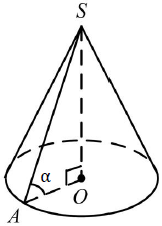
\includegraphics[width=\textwidth]{vbe2017_24.png}
\end{minipage}
\item[]
\begin{minipage}[b]{0.8\linewidth}
\item Stačiojo trikampio įžambinės ilgis yra lygus $c$, o statinių ilgiai yra lygūs $a$ ir $b$. Vienas iš kampų, esančių prie statinių, lygus $\alpha$. 
\begin{tasks}(1)
\task Kiek kartų reikia sumažinti trikampio kraštines, kad trikampio įžambinės ilgis būtų lygus 1?
\task Kam lygūs sumažinto trikampio statiniai?
\task Ar pakito $\alpha$ reikšmė sumažinus trikampį?
\task Patalpinkite sumažintą trikampį trigonometriniame skritulyje. Kam lygios reikšmės $\sin{\alpha}$ ir $\cos{\alpha}$?
\end{tasks}
\end{minipage}
\begin{minipage}[b]{0.2\linewidth}
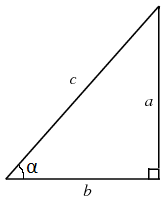
\includegraphics[width=\textwidth]{transtriangle.png}
\end{minipage}
\begin{minipage}[b]{0.77\linewidth}
\item (VBE 2014, 22) Metalinį 2 m ilgio strypą sulenkė tiksliai per vidurį taip, kad tarp
strypo dalių susidarė 120° kampas. Koks atstumas tarp sulenkto
strypo galų? Atsakymą suapvalinkite iki centimetrų. \textit{Pastaba:} $\sqrt{3}\approx 1,73205$
\end{minipage}
\begin{minipage}[b]{0.23\linewidth}
\includegraphics[width=\textwidth]{vbe2014_22.png}
\end{minipage}
\save
\end{enumerate}
\end{mdframed}


\subsection{Laipsnių vertimas į radianus}
\edef\myindent{\the\parindent}
\begin{minipage}[b]{0.7\linewidth}
\setlength{\parindent}{\myindent}
Vienas iš sunkumų pereinant nuo paprastos geometrijos prie trigonometrijos yra tai, jog geometrinių figūrų kampus įprasta išreikšti laipsniais, o trigonometriniame skritulyje kampai gali būti išreikšti ir laipsniais, ir radianais. Jei norime paversti tam tikrą kampą radianais, imame tą kampą atitinkančio lanko ilgį vienetiniame skritulyje. Pavyzdžiui vienetiniame skritulyje 180° kampą atitinka $\pi$, nes 180° kampą atitinkančio lanko ilgis tame skritulyje yra $\pi$. Atitiktį tarp laipsnių ir jų radianų galima pavaizduoti lentele:

\begin{tabular}{|c||c|c|c|c|c|c|c|c|}
\hline 
Laipsniai & 0° & 30° & 45° & 60° & 90° & 180° & 270° & 360° \\ \hline
Radianai & $\begin{array}{c}\phantom{0} \\ 0 \\ \phantom{0} \end{array}$ & $\displaystyle\frac{\pi}{6}$  & $\displaystyle\frac{\pi}{4}$ & $\displaystyle\frac{\pi}{3}$ & $\displaystyle\frac{\pi}{2}$ & $\pi$ & $\displaystyle\frac{3\pi}{2}$ & $2\pi$ \\ \hline
\end{tabular}
\end{minipage}
\begin{minipage}[b]{0.25\linewidth}
\includegraphics[width=\textwidth]{"radianus".png}
\end{minipage} 
\newpage
\begin{mdframed}[backgroundcolor=blue!10!white, linewidth=3pt]
\begin{enumerate}
\resume
\hitem{https://www.wolframalpha.com/input/?i=150+degrees} Išreikškite 1°, 20° ir 220° kampus radianais.
\hitem{https://www.wolframalpha.com/input/?i=pi\%2F9} Išreikškite $\frac{\pi}{180}$, $\frac{\pi}{10}$ ir $\frac{\pi}{5}$ kampus laipsniais.
\end{enumerate}
\end{mdframed}

\subsection{Kitų nesudėtingų kampų trigonometrinių funkcijų radimas}
Ankstesnėse dalyse matėme kaip nustatyti $\cos\text{30°}$, $\cos$ 45°, $\cos$ 60°, $\sin$ 30°, $\sin$ 45°, $\sin$ 60° ir reikšmes. Pagal apibrėžimus $\text{tg}a=\frac{\sin a}{\cos a}$ ir $\text{ctg}a=\frac{\cos a}{\sin a}$ galima nustatyti ir tų pačių kampų tangentus bei kotangentus. Lieka neaišku, kaip nustatomos likusių kampų trigonometrinės funkcijos.
\begin{enumerate}
\begin{minipage}[b]{0.65\linewidth}
\item Kampų 10°, 15°, 36° ir t.t. trigonometrinių funkcijų reikšmės įgyja sudėtingesnes formas. Pavyzdžiui $\cos 36^o = \frac{1+\sqrt{5}}{4}$. Tokioms reikšmėms gauti reikia remtis trigonometrinėmis tapatybėmis, kurias aptarsime antrame skyriuje.
\item Kampai 120°, 135°, 150° (antras ketvirtis), 210°, 225°, 240° (trečias ketvirtis) ir 300°, 315°, 330° (ketvirtas ketvirtis) yra 30° arba 45° kartotiniai, todėl kuriame nors trigonometrinio skritulio ketvirtyje atskelia trečdalį arba pusę. Jie atitinka parodytus spindulio pasukimus trigonometriniame skritulyje. Dėl šios savybės šiuos kampus laikome nesudėtingais. Jų funkcijų reikšmes apskaičiuoti taip pat galime, jei remsimės tokiu dėsningumu:
\end{minipage}
\begin{minipage}[b]{0.35\linewidth}
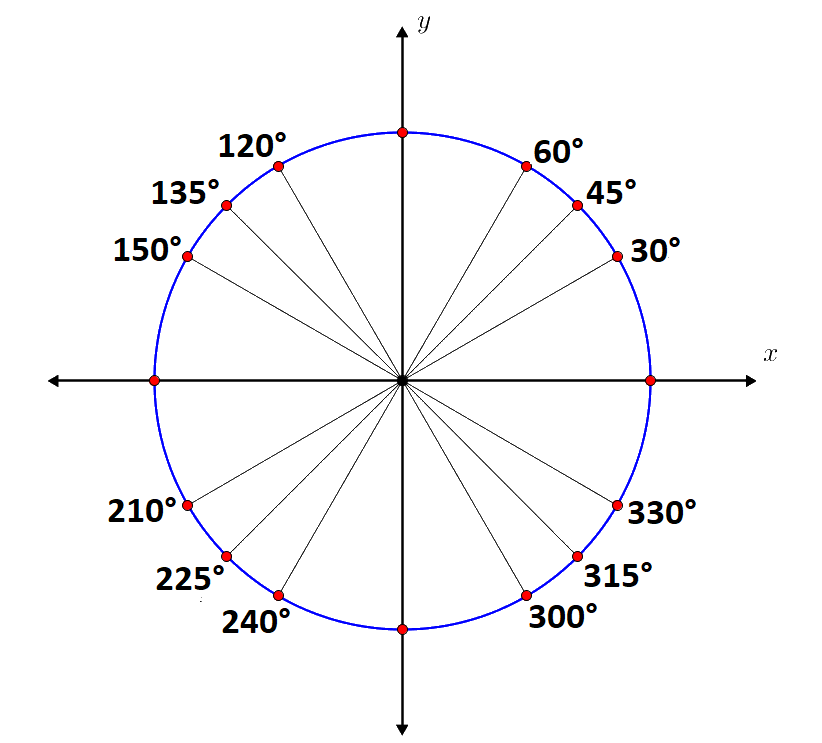
\includegraphics[width=\textwidth]{easy_angles.png}
\end{minipage}
\end{enumerate}
\begin{mdframed}[backgroundcolor=yellow!50!white]
Kiekvieno nesudėtingo kampo sinusai bei kosinusai yra lygūs skaičiams $\pm \frac{1}{2}$, $\pm \frac{\sqrt{2}}{2}$ ir $\pm \frac{\sqrt{3}}{2}$.
\end{mdframed}

Kodėl tai galioja išsiaiškinsime kitame poskyryje
\begin{mdframed}[backgroundcolor=blue!10!white, linewidth=3pt]
Pateiktuose paveikslėliuose taškai, gauti trigonometrinio skritulio spindulį nukreipiant kampais 

$\text{30°, 45°, ... , 330°}$, yra sujungti žaliomis atkarpomis kaip parodyta.

\begin{minipage}[b]{0.45\linewidth}
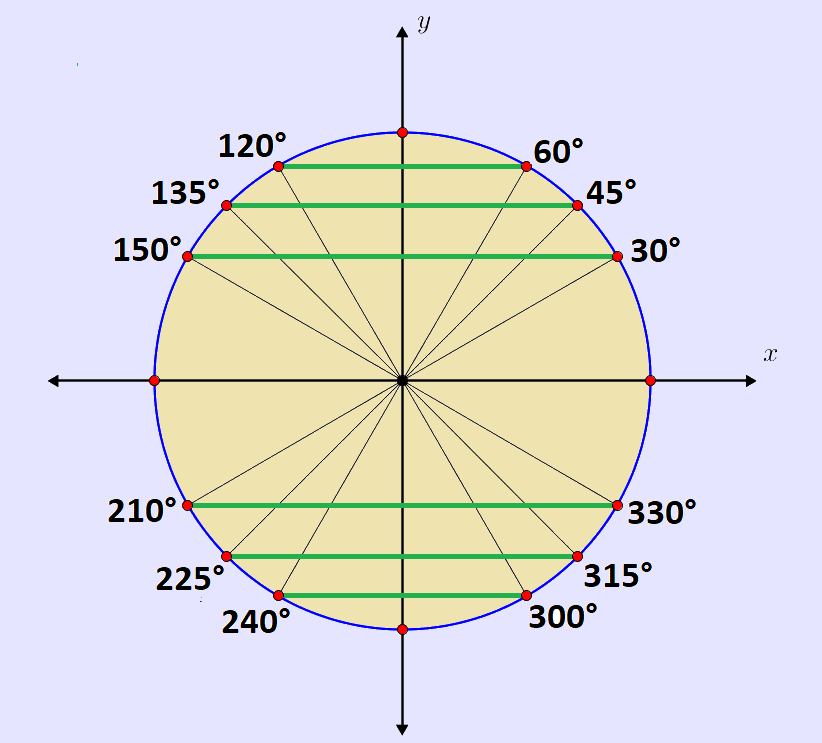
\includegraphics[width=\textwidth]{hlevels.png}
\end{minipage}
\begin{minipage}[b]{0.45\linewidth}
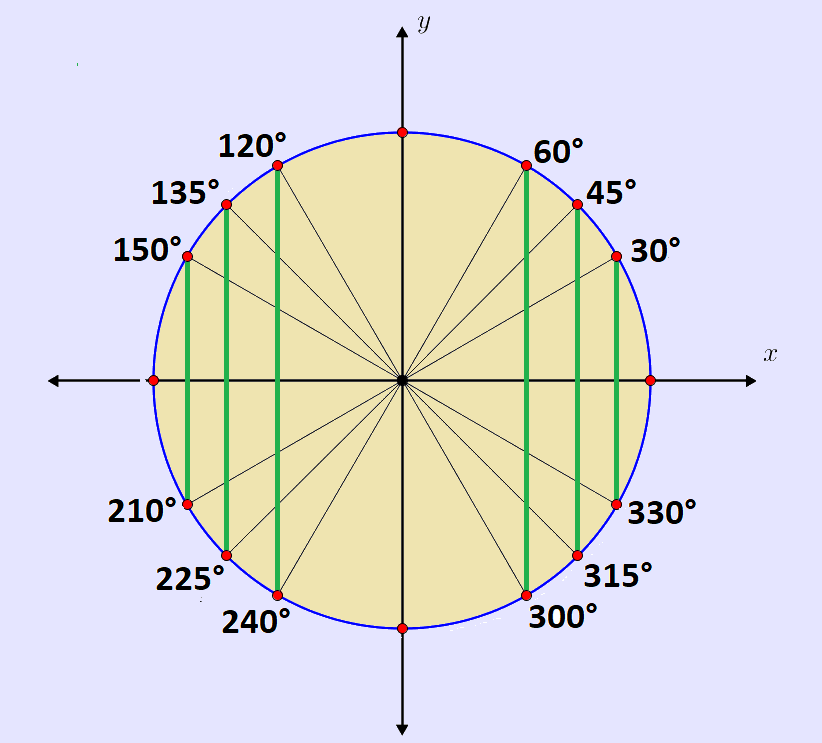
\includegraphics[width=\textwidth]{vlevels.png}
\end{minipage}
\begin{enumerate}
\resume
\item Paaiškinkite, kodėl pirmame paveikslėlyje žalios atkarpos yra lygiagrečios $x$ ašiai, o antrame $y$ ašiai.
\item Remdamiesi dėsningumu didėjimo tvarka nurodykite:
\begin{tasks}(1) 
\task ordinates visų taškų, priklausančių pirmojo paveikslėlio žalioms atkarpoms
\task abscises visų taškų, priklausančių antrojo paveikslėlio žalioms atkarpoms
\end{tasks}
(abiejų dalių atsakymas vienodas)
\item Remdamiesi paveikslėliais išrašykite visas juose pavaizduotų kampų $\alpha$ ir $\beta$ poras, tokias, kad 
\begin{tasks}(2) 
\task $\sin{\alpha}=\sin{\beta}$
\task $\cos{\alpha}=\cos{\beta}$
\end{tasks}
\item Remdamiesi antruoju paveikslėliu paaiškinkite, kodėl $\cos(x)=\cos(-x)$ kiekvienam $x$.
\item Teisingai atlikus pratimą su kampų poromis galima pastebėti, jog $\sin(\text{90°}+x)=\sin(\text{90°}-x)$, kai $x$ lygus 30°, 45°, 60°, 120°, 135°, 150°. Iš tiesų ši lygybė galioja su visais kampais $x$. Remdamiesi pirmu brėžiniu pamėginkite apibūdinti kampo $x$ prasmę.
\end{enumerate}
\end{mdframed}

Kitas skyrius - redukcijos formulės

\begin{mdframed}[backgroundcolor=blue!10!white, linewidth=3pt]
\begin{enumerate}
\hitem{} Naudodamiesi BRĖŽINIU apskaičiuokite trigonometrinių funkcijų reikšmes
\begin{tasks}(5)
\task $\sin{\frac{\pi}{3}}$
\task $\sin{\frac{\pi}{2}}$
\task $\sin{\frac{\pi}{4}}$
\task $\cos{\frac{\pi}{4}}$
\task $\text{tg}{\frac{\pi}{4}}$
\task $\text{tg}{\frac{\pi}{3}}$
\task $\sin{\frac{2\pi}{3}}$
\task $\sin{\left(-\frac{2\pi}{3}\right)}$
\task $\cos{\frac{2\pi}{3}}$
\task $\sin{\frac{3\pi}{2}}$
\task $\sin{\left(-\frac{3\pi}{2}\right)}$
\task $\cos{\frac{2\pi}{3}}$
\task $\cos{\left(-\frac{2\pi}{3}\right)}$
\task $\text{*tg}\frac{7\pi}{4}$
\end{tasks}
\end{enumerate}
\end{mdframed}

\subsection{Trigonometrinių funkcijų GRAFIKAI}
Pavaizduosime, kaip pasinaudojant BRĖŽINIU yra gaunami trigonometrinių funkcijų grafikai.
\newpage
\begin{center}$f(x)=\sin(x)$\end{center}
\pgfmathsetmacro\myangle{0}
\def\angle{\myangle}
\begin{animateinline}[controls,autoplay,loop]{15}
\whiledo{\lengthtest{\angle pt<360pt}}{%
  \begin{tikzpicture}
    % fill circle and plot
    \fill[blue!50] (-1,0) arc (0:\angle:2) -- (-3,0) -- cycle; %goes to; startangle:initialangle:radius; goes from
    \fill[blue!50] plot[smooth,domain=0:\angle] (pi/180*\x,{2*sin(\x)}) |- (0,0);
    % draw connection
    \draw (-3,0) +(\angle:2) circle (4pt) -- (pi/180*\angle,{2*sin(\angle)}) circle (4pt);
    % draw axes an ticks
    \draw (-5.5,0) -- (7,0);
    \foreach \deg in {45,90,135,180,225,270,315,360}
      \draw (pi/180*\deg,2pt) -- (pi/180*\deg,-2pt) node[below] {$\deg^\circ$};
    \draw (0,-2.2) -- (0,2.2);
    \foreach \y in {-1,-0.5,0.5,1}
      \draw (2pt,2*\y) -- (-2pt,2*\y) node[left] {$\y$};
    %draw blue stick
    \draw[very thick, blue] (-3,0) +(\angle:2) circle (4pt) -- (-3,0);
    % draw plot and circle outline
    \draw plot[smooth,domain=0:360] (pi/180*\x,{2*sin(\x)});
    \draw (-3,0) circle (2);%
   \pgfmathsetmacro\myangle{\angle+5.0} %myangle cant be used globally
   \xdef\angle{\myangle} %we copy it to global variable
   \end{tikzpicture}
   \ifthenelse{\lengthtest{\angle pt<360pt}}{\newframe}{\end{animateinline}}   
}


\begin{center}$f(x)=\cos(x)$\end{center}

\pgfmathsetmacro\myangle{0}
\xdef\angle{\myangle}
\begin{animateinline}[controls,autoplay,loop]{15}
\whiledo{\lengthtest{\angle pt<360pt}}{%
  \begin{tikzpicture}
    % fill circle and plot
    \fill[blue!50] (-3,2) arc (90:\angle+90:2) -- (-3,0) -- cycle; %goes to; startangle:initialangle:radius; goes from
    \fill[blue!50] plot[smooth,domain=0:\angle] (pi/180*\x,{2*cos(\x)}) |- (0,0);
    % draw connection
    \draw (-3,0) +(\angle+90:2) circle (4pt) -- (pi/180*\angle,{2*cos(\angle)}) circle (4pt);
    % draw axes an ticks
    \draw (-5.5,0) -- (-5,0);
    \draw (-1,0) -- (7,0);
    \draw (-3,-2) -- (-3,2);
    \foreach \deg in {45,90,135,180,225,270,315,360}
      \draw (pi/180*\deg,2pt) -- (pi/180*\deg,-2pt) node[below] {$\deg^\circ$};
    \draw (0,-2.2) -- (0,2.2);
    \foreach \y in {-1,-0.5,0.5,1}
      \draw (2pt,2*\y) -- (-2pt,2*\y) node[left] {$\y$};
    %draw blue stick
    \draw[very thick, blue] (-3,0) +(\angle+90:2) circle (4pt) -- (-3,0);
    % draw plot and circle outline
    \draw plot[smooth,domain=0:360] (pi/180*\x,{2*cos(\x)});
    \draw (-3,0) circle (2);%
   \pgfmathsetmacro\myangle{\angle+5.0} %myangle cant be used globally
   \xdef\angle{\myangle} %we copy it to global variable
   \end{tikzpicture}
   \ifthenelse{\lengthtest{\angle pt<360pt}}{\newframe}{\end{animateinline}}   
}
\newpage
\begin{center}$f(x)=\text{tg}(x)$\end{center}

\pgfmathsetmacro\myangle{0}
\xdef\angle{\myangle}
\begin{animateinline}[controls,autoplay,loop]{15}
\whiledo{\lengthtest{\angle pt<360pt}}{%
  \begin{tikzpicture}
    % fill circle and plot
    \path[use as bounding box] (-5.6,-4.7) rectangle (6.6,4.7);
    \ifthenelse{\lengthtest{\angle pt=90pt}}{}{
    \ifthenelse{\lengthtest{\angle pt=270pt}}{}{
    \fill[blue!50] plot[smooth,domain=0:1.5] (\x-3,{\x*tan(\angle)}) |- (0,0); %goes to; startangle:initialangle:radius; goes from
    \ifthenelse{\lengthtest{\angle pt<90pt}}{\fill[blue!50] plot[smooth,domain=0:\angle] (pi/180*\x,{1.5*tan(\x)}) |- (0,0);}{
    \fill[blue!50] plot[smooth,domain=0:85] (pi/180*\x,{1.5*tan(\x)}) |- (0,0);
     \ifthenelse{\lengthtest{\angle pt<270pt}}{\fill[blue!50] plot[smooth,domain=95:\angle] (pi/180*\x,{1.5*tan(\x)}) |- (9.5*pi/18,0);}{
     \fill[blue!50] plot[smooth,domain=100:265] (pi/180*\x,{1.5*tan(\x)}) |- (9.5*pi/18,0);
     \fill[blue!50] plot[smooth,domain=275:\angle] (pi/180*\x,{1.5*tan(\x)}) |- (27.5*pi/18,0);}}
    % draw connection
    \draw (-1.5,{1.5*tan(\angle)}) circle (3pt) -- (pi/180*\angle,{1.5*tan(\angle)}) circle (3pt);}}
    % draw axes an ticks
    \draw (-5.5,0) -- (7,0);
    \foreach \deg in {45,90,135,180,225,270,315,360}
      \draw (pi/180*\deg,2pt) -- (pi/180*\deg,-2pt) node[below] {$\deg^\circ$};
    \draw (0,-7.6) -- (0,7.6);
    \foreach \y in {-5,-4,-3,-2,-1,-0.5,0.5,1,2,3,4,5}
      \draw (2pt,1.5*\y) -- (-2pt,1.5*\y) node[left] {$\y$};
    %draw blue stick
    \draw[very thick, blue] (-3,0) +(\angle:1.5) -- (-3,0);
    % draw plot and circle outline
    \draw plot[smooth,domain=0:80] (pi/180*\x,{1.5*tan(\x)});
    \draw plot[smooth,domain=100:260] (pi/180*\x,{1.5*tan(\x)});
    \draw plot[smooth,domain=280:360] (pi/180*\x,{1.5*tan(\x)});
    \draw (-3,0) circle (1.5);%
   \pgfmathsetmacro\myangle{\angle+5.0} %myangle can't be used globally
   \xdef\angle{\myangle} %we copy it to global variable
   \end{tikzpicture}
   \ifthenelse{\lengthtest{\angle pt<360pt}}{\newframe}{
   \end{animateinline}
   }   
}

\subsection{Atvirkštinės funkcijos}
Trigonometrinių funkcijų $\sin x$, $\cos x$ ir $\text{tg} x$ atvirkštinės funkcijos $\arcsin x$, $\arccos x$ ir $
\arctan x$ yra apibrėžiamos taip:

\tcbset{highlight math style={enhanced,
  colframe=red!60!black,colback=yellow!50!white,arc=4pt,boxrule=1pt}} %highlight of equations
  
\begin{empheq}[box=\tcbhighmath]{align*}
\Aboxed{x=\sin y, & y \in \left[-\frac{\pi}{2}, \frac{\pi}{2}\right]} & \Leftrightarrow & \Aboxed{y=\arcsin x}\\
\Aboxed{x=\cos y, & y \in \left[0,\pi\right]} & \Leftrightarrow & \Aboxed{y=\arccos x}\\
\Aboxed{x=\text{tg} y, & y \in \left[-\frac{\pi}{2},\frac{\pi}{2}\right]} & \Leftrightarrow & \Aboxed{y=\arctan x}\\
\end{empheq}

Intervalai, kuriuose kinta $y$, yra specialiai parinkti taip, kad funkcijos $\sin y$, $\cos y$ ir $\text{tg} y$ dukart neįgytų tos pačios reikšmės. \textbf{Tik tokiu atveju jos gali turėti atvirkštines funkcijas.}

\begin{enumerate}
\item Naudodamiesi BRĖŽINIU arba trigonometrinių funkcijų GRAFIKAIS raskite visus kampus $x$ intervale $[0,2\pi]$, tokius, kad:
\begin{tasks}(3)
\task $\sin{x}=1$
\task $\cos{x}=1$
\task $\sin{x}=0$
\task $\cos{x}=0$
\task $\text{tg}{x}=1$
\task $\text{ctg}{x}=1$
\task $\sin{x}=\frac{\sqrt{2}}{2}$
\task $\cos{x}=\frac{\sqrt{2}}{2}$
\task $\sin{x}=0,5$
\task $\cos{x}=0,5$
\task $\sin{x}=\frac{\sqrt{3}}{2}$
\task $\cos{x}=\frac{\sqrt{3}}{2}$
\task $\text{tg}{x}=\frac{\sqrt{3}}{3}$
\task $\text{ctg}{x}=\frac{\sqrt{3}}{3}$
\end{tasks}
\item Pasinaudosime šio skyrelio žiniomis

$\begin{cases}sin^2x+cos^2x=1 \\ \sin\text{ ir }\cos \text{ geometrinė interpretacija} \end{cases}$ 

bei ankstesnėmis žiniomis 

$\begin{cases}\text{greitosios daugybos formulė }(a-b)^2=a^2-2ab+b^2 \\ \text{Pitagoro teorema } c^2=a^2+b^2\end{cases}$ 

ir įrodysime Kosinusų Teoremą \fbox{$c^2=a^2+b^2-2ab\cos{C}$}.

\includegraphics[width=0.5\textwidth]{"lawofcosines".png}

Remdamiesi brėžiniu paaiškinkite:
\begin{itemize}
\item Kodėl trikampio aukštinė yra lygi $a\sin C$? (BRĖŽINYS)
\item Kodėl dešinioji pagrindo dalis yra lygi $a\cos C$? (BRĖŽINYS)
\item Kodėl kairioji pagrindo dalis yra lygi $b-a\cos C$?
\item Kodėl tenkinama lygybė $c^2=(a\sin C)^2+(b-a\cos C)^2$?
\item Įrodykite tapatybę $(a\sin C)^2+(b-a\cos C)^2=a^2+b^2-2ab\cos{C}$ (FORMULĖ $(a-b)^2$)
\end{itemize}
\item \tbf{Bonus}. Įrodykite Herono formulę: bet kurio trikampio su kraštinėmis $a, b, c$ ir pusperimetriu $p$ plotas $S=\sqrt{p(p-a)(p-b)(p-c)}$. Galite remtis išvada $S=\frac{ab\sin C}{2}=\frac{ab\sqrt{1-\cos^2C}}{2}$
\end{enumerate}
\newpage
\section{Antra pamoka}
\begin{mdframed}[backgroundcolor=yellow!50!white]
\begin{itemize}
\item $\sin(x+y)=\sin{x}\cos{y}+\sin{y}\cos{x}\quad \stackrel{y \to x}{\Rightarrow} \quad \sin 2x = 2\sin x \cos x$
\item $\cos(x+y)=\cos{x}\cos{y}-\sin{x}\sin{y}\quad \stackrel{y \to x}{\Rightarrow} \quad \cos 2x = \cos^2x-\sin^2y$
\end{itemize}
\end{mdframed}
Kaip galima greitai gauti kampų sumos formules? Galite pasinaudokite egzaminų lapu arba atsiminti tokiu būdu: 
\begin{itemize}
\item Tapatybes $\begin{cases}\sin 2x = 2\sin x \cos x \\ \cos 2x = \cos^2x-\sin^2y\end{cases}$ įsiminti šiaip ar taip teks
\item Parašome: $\begin{cases}\sin (x+x) = \sin x \cos x+\sin x \cos x \\ \cos (x+x) = \cos x\cos x-\sin x \sin x\end{cases}$
\item Šiose išraiškose pasirenkame narius $\sin x$ ir $\cos x$, ir pakeičiame į $\sin y$ ir $\cos y$ taip, kad naujoji išraiška nebūtų suprastinama:

\fbox{$\begin{array}{cc}
\sin x \cos x+\sin x \cos x & \rightarrow \\
\sin x \cos y+\sin y \cos x &      
\end{array}$} ir 
\fbox{$\begin{array}{cc}
\cos x \cos x-\sin x \sin x & \rightarrow \\
\cos x \cos y-\sin x \sin y &     
\end{array}$}
\end{itemize}

\begin{enumerate}
\item Kampų sumos formulėse įstatykite $y \rightarrow -y$ ir jas pertvarkykite į kampų skirtumo formules:
\begin{tasks}
\task $\sin(x-y)$
\task $\cos(x-y)$
\end{tasks}
\item Pasinaudoję tangento apibrėžimu (pirma pamoka) bei kampų sumos formulėmis, įrodykite, kad 
$$\text{tg}(x+y)=\frac{\text{tg} x+\text{tg} y}{1-\text{tg} x\text{tg} y}$$
\item \tbf{Bonus!} Sudėkite $\sin(x-y)$ ir $\sin(x+y)$ formules, pakeiskite $\begin{cases} x-y=A \\ x+y=B\end{cases}$, įsitikinkite, kad galioja $$\begin{cases}x-y=A \\ x+y=B\end{cases} \leftrightarrow \begin{cases}x=\frac{A+B}{2} \\ y=\frac{B-A}{2}\end{cases}$$ ir pasinaudoję pakeitimu išveskite reiškinio formulę \fbox{$\sin A + \sin B=2\sin\left(\frac{B+A}{2}\right)\cos\left(\frac{B-A}{2}\right)$}
\item \tbf{Bonus!} Sudėkite $\cos(x-y)$ ir $\cos(x+y)$ formules, pakeiskite $\begin{cases} x-y=A \\ x+y=B\end{cases}$, įsitikinkite, kad galioja $$\begin{cases}x-y=A \\ x+y=B\end{cases} \leftrightarrow \begin{cases}x=\frac{A+B}{2} \\ y=\frac{B-A}{2}\end{cases}$$ ir pasinaudoję pakeitimu išveskite reiškinio formulę \fbox{$\cos A + \cos B=2\cos\left(\frac{B+A}{2}\right)\cos\left(\frac{B-A}{2}\right)$}
\item Egzamino uždavinys (sunkus): išspręskite lygtį $\sin x = \cos 75^o+\cos 15^o$
\item \tbf{Bonus!} Sinusoide yra vadinama funkcija, kurią galime parašyti kaip $k\sin{ax+b}$ (arba $k\cos{ax+b}$). Įrodysime, kad visos funkcijos, užrašomos forma $a\sin x + b\cos x$, yra sinusoidės.
\begin{itemize}
\item Pakeiskite reiškinį į $\sqrt{a^2+b^2} \cdot \left(\frac{a}{\sqrt{a^2+b^2}}\sin x + \frac{b}{\sqrt{a^2+b^2}}\cos x\right)$
\item Parodykite, kad skaičiai $X=\frac{a}{\sqrt{a^2+b^2}}$ ir $Y=\frac{b}{\sqrt{a^2+b^2}}$ tenkina $X^2+Y^2=1$, kas reiškia, jog $X$ ir $Y$ visada gali būti to paties kampo sinusas ir kosinusas:

$\begin{cases}X=\cos t \\ Y=\sin t \end{cases}$
\item Kam lygus reiškinys $\cos t \sin x + \sin t \cos x$?
\end{itemize}
\item Panaudokite formulę $\boxed{\sin \alpha \cos \beta=\frac{1}{2}\left(\sin (\alpha-\beta)+\sin (\alpha+\beta)\right)}$ reiškiniui

 $2\sin(4\alpha)\cos(2\alpha) - \sin(6\alpha)$ suprastinti.
\end{enumerate}
\end{document}